\chapter{Fundamentação Teórica}
Para dar ínicio ao nosso panorama geral revisaremos, neste capítulo, os conceitos básicos sobre som, o que é informação musical e como é feito o armazenamento no banco de dados, quais as representações e estruturas do áudio digital e por fim, a recuperação da informação musical.

\section{Conceitos Básicos sobre Som}
Nós ouvimos uma variedade de sons à todo momento, e vivemos toda a nossa vida rodeados por eles. Sons de portas abrindo e fechando, dos passos, do ruído dos motores dos automóveis, da chuva e da música. O som não é algo que podemos ver com nossos olhos. Então, o que é o som? Usando o exemplo do som de uma campainha, temos que quando a energia cinética é aplicada a ela, através de um martelo, ocorre uma “deformação” da campainha, gerando desta maneira a energia que trata de devolver a campainha ao seu estado original. Começa, então, uma repetição periódica de deformações e restaurações. A isto chamamos de vibração. Estas vibrações produzem mudanças de pressão do ar, resultando em seções de ar que são mais densas e outras que são rarefeitas, ocorrendo sucessivamente uma depois da outra e expandindo-se. Estas são chamadas condensações e rarefações. O processo é similar ao que conhecemos quando jogamos uma pedra dentro d’água, a qual produz ondas circulares em sua superfície. Estas ondas de condensações e rarefações são propagadas para dentro do ouvido humano e irão vibrar o tímpano. As vibrações são captadas pelas terminações nervosas, de maneira que nós as escutamos como sons. Se os corpos que vibram são diferentes, também será diferente a classe de vibração que produzem, isto significa que escutamos distintas classes de sons. No espaço, onde não existe ar, também não existem sons \cite{miletto2004}.

Os autores explicam que o som, é, portanto, a vibração do ar, ou seja, variações na pressão do ar, que percebemos com nossos ouvidos. Se essa pressão varia de acordo com um padrão repetitivo dizemos que o som tem uma forma de onda periódica. Se não há um padrão perceptível no som este é chamado de ruído. E quando as variações na pressão do ar são representadas de forma gráfica, podem ser interpretadas como “formas de onda”. Na Figura \ref{fig:ondaSenoidal} a representação gráfica de um som mostra as mudanças na pressão do ar conforme a passagem do tempo. Lendo-se o gráfico da esquerda para a direita, quando a linha curva está próxima da parte inferior do gráfico, então a pressão do ar é mais baixa, e quando a curva está próxima do topo do gráfico, a pressão do ar aumentou.

\begin{figure}[!htb]
   \centering
   \caption{Representação gráfica, no domínio temporal, de uma forma de onda senoidal}\label{fig:ondaSenoidal} 
   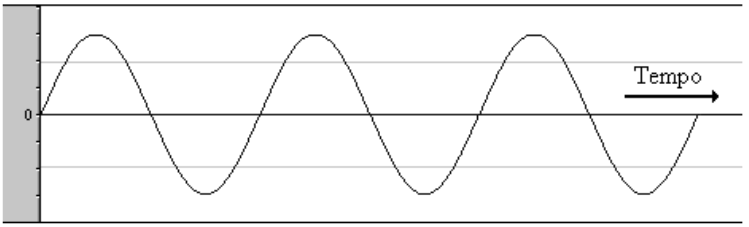
\includegraphics[scale=0.4]{figuras/ondaSenoidal.png}
   Fonte: \cite{miletto2004}.
\end{figure}

\citeonline{miletto2004} apresentam os quatro elementos básicos do som, que são:
\begin{enumerate}
\item Altura tonal \newline
Quando se toca as teclas de um piano, nota-se que os sons são mais agudos quanto mais tocados à direita e mais graves quanto mais se tocar à esquerda. Essa “altura” de um som, ou seja, se é alto ou baixo, agudo ou grave, é chamada “altura tonal”.

Uma repetição de uma onda periódica é chamada de ciclo. Quanto mais agudo o som, maior o número de ciclos por unidade de tempo e quanto mais grave o som, menor será este número. O número de ciclos dentro do intervalo de um segundo é geralmente chamado freqüência e expresso em unidades chamadas hertz (Hz). 100Hz indica que a vibração ocorre com uma freqüência de 100 ciclos por segundo. Quanto maior o valor em hertz, mais agudo é o som. Dobrando a freqüência de um som, este é elevado em uma oitava, então é possível dizer que a freqüência e a altura tonal estão relacionadas logaritmicamente. A faixa de freqüências que podem ser ouvidas por um ouvido humano é de aproximadamente 20Hz para os sons mais graves e de até 20.000Hz para os sons mais agudos.

\item Volume \newline
Se uma tecla de piano é pulsada fortemente, o som produzido será forte. Se for pulsada suavemente, o som produzido será fraco. As denominações alto e baixo devem ser utilizadas de maneira correta apenas para designar a altura tonal e não o volume. A mudança no volume de um som pode ser vista como uma diferença na altura das ondas. A altura de uma onda chama-se “amplitude”. Quanto maior a amplitude, mais forte é o som. Portanto o volume de um som é determinado pela amplitude (altura da onda). Ao contrário do que é falado coloquialmente, um som alto, do ponto de vista da amplitude corresponde a um som forte. Já um som baixo, corresponde a um som fraco.

\item Timbre \newline
Um clarinete e uma flauta não produzem o mesmo som ao serem tocados com a mesma altura tonal e o mesmo volume. Isso se deve ao fato de haver um fator distinto a mais para o som além da altura tonal e do volume. Este fator é o timbre. De um modo geral, formas de ondas arredondadas produzem um timbre mais suave enquanto que as formas de ondas ponteagudas dão um timbre mais penetrante e estridente.

Na Figura \ref{fig:ondaTimbre} são mostradas três formas de onda básicas, seus timbres característicos e os instrumentos que se assemelham a cada caso.

\begin{figure}[!htb]
   \centering
   \caption{Formas de onda simples e seus timbres}\label{fig:ondaTimbre} 
   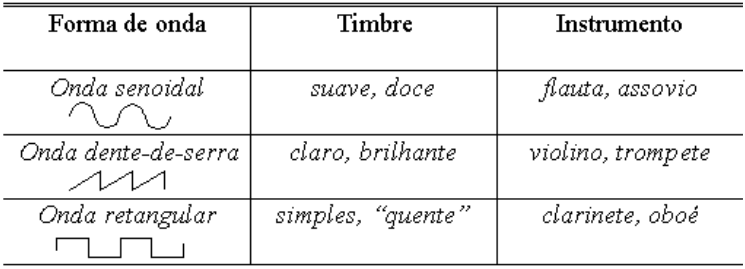
\includegraphics[scale=0.4]{figuras/ondaTimbre.png}
   Fonte: \cite{miletto2004}.
\end{figure}

\item Envolvente da Onda \newline
Trata-se da variação do som em um transcurso de tempo. Mais precisamente, a variação de cada um dos três elementos em um transcurso de tempo que vai desde o começo do som até um ponto do tempo onde ele desaparece completamente. Se um violino for tocado com arco, por exemplo, geralmente o volume do som aumenta gradualmente e também o timbre e a altura tonal mudam ligeiramente. Estas mudanças no tempo são o que determina o timbre característico de um violino, além do seu espectro harmônico. Por outro lado, o relaxamento do som de um piano é um caimento contínuo. Sem este caimento seria muito difícil distingüi-lo do som de uma flauta. Envolventes são, portanto, as mudanças de altura tonal, volume e timbre em um transcurso de tempo. Ocasionalmente, a mudança apenas do volume (amplitude) em um transcurso de tempo é também chamada envolvente.
\end{enumerate}

Segundo \citeonline{miletto2004} é possível encontrar dois tipos de sons: Sons Complexos e Sons Harmônicos ou Parciais.

Os sons complexos são formados por ondas simples (ondas senoidais) que são os harmônicos e a fundamental. Os harmônicos ou parciais são múltiplos da freqüência básica ou fundamental. A fundamental de um som complexo é o componente de mais baixa freqüência. A freqüência fundamental e seus harmônicos constituem a série harmônica. A resultante é uma forma de onda que representa um som complexo.

E o som é dividido em sons musicais e não-musicais dependendo do tipo de vibração principal. Os sons com vibrações regulares (ou seja, sons em que existem muito poucos componentes distintos dos harmônicos) são considerados musicais, enquanto os sons causados por vibrações irregulares complicadas (ou seja, sons com muitos componentes que não são harmônicos), cuja altura tonal não pode, portanto, ser medida, são chamados sons não-musicais. Os sons não-musicais incluem também os sons do tipo desagradáveis. A maioria dos sons usados na música são, por pressuposto, sons musicais. Várias classes de ruídos, como os produzidos por instrumentos de percussão, são também usados para realizar o efeito musical.

\section{Informação Musical}
Para \citeonline{miletto2004} o processo de representar numericamente o som é chamado de digitalização. Um som contendo freqüências limitadas pode então ser representado por uma seqüência de simbolos quantificados ou quantificáveis, ou seja, de números. Segundo \citeonline{setzer2001}, dado é uma sequencia de números, portanto, um texto, fotos, figuras, sons gravados e animação são dados, pois todos podem ser quantificados. Um dado é necessariamente uma entidade matemática e, desta forma, é puramente sintático. Isto significa que os dados podem ser totalmente descritos através de respresentações formais, estruturais e obviamente ser armazenados em um computador e processados por ele. O processamento de dados em um computador limita-se exclusivamente a manipulações estruturais dos mesmos, e é feito por meio de programas. Estes são sempre funções matemáticas, e portanto também são dados. Exemplos dessas manipulações nos casos de textos são a comparação com outros textos, etc.

Sendo o dado puramente sintático, ao incluir um “significado” implícito na palavra, usado para sua caracterização, é gerado a informação, que é necessariamente semântica.

O autor expõe que a informação é uma abstração informal (isto é, não pode ser formalizada através de uma teoria lógica ou matemática) que está na mente de alguém, representando algo significativo para essa pessoa. Utilizando-se da frase “Paris é uma cidade fascinante” é um exemplo de informação – desde que seja lida ou ouvida por alguém, desde que "Paris" signifique para essa pessoa a capital da França (supondo-se que o autor da frase queria referir-se a essa cidade) e "fascinante" tenha a qualidade usual e intuitiva associada com essa palavra.

A informação pode ser armazenada em um computador, ou melhor, a sua representação em forma de dados e não a informação propriamente dita. Essa representação pode ser transformada pela máquina, como na formatação de um texto (o que seria uma transformação sintática), mas não pode mudar o significado, já que ele depende de uma pessoa que possui a informação. Os dados são sempre incorporados por alguém como informação, porque os seres humanos buscam constantemente por significação e entendimento \citeonline{setzer2001}.

Á partir daí, a autora \citeonline{barros2012} expõe que um dado musical é resultado de um processo de significação social. Assim, a música é uma expressão humana construída socialmente e objetivada por meio de sua comunicação oral, registro sonoro ou representação gráfica.

Para \citeonline{almeida2007}, a obra musical é efêmera e abstrata, pois só se concretiza no momento de cada interpretação, na execução da música. \citeonline{berger&luckmann2014} afirmam que:

\begin{citacao}
A expressividade humana é capaz de objetivações, isto é, manifesta-se em produtos da atividade humana que estão ao dispor tanto dos produtores quanto dos outros homens, como elementos que são de um mundo comum.
\end{citacao}

Para \citeonline{angeles2010,pinheiro&loureito1995} a informação é o que se acrescenta a uma representação. Segundo o autor, recebemos informação se o que conhecemos é alterado. Informação é o que logicamente justifica alteração ou reforço de uma representação ou de um estado de coisas. As representações podem ser explícitas (como em um mapa, ou em uma proposição), ou podem estar implícitas no estado de atividade dirigida do receptor.

A informação musical apresenta determinadas especificidades de comportamento na sua produção, objetivação e uso, pois a manifestação da música apresenta-se carregada de características próprias. \citeonline{michels1992} explica que a música contém dois elementos: o material acústico e a ideia intelectual, sendo que tais elementos não se encontram justapostos, mas sim, se combinam para formar uma imagem unitária. Portanto, a compreensão completa da música está diretamente ligada com o reconhecimento do contexto histórico e social de sua origem, com a interpretação pessoal e individual do ouvinte, e com os aspectos sonoros que a constituem, dessa forma, a música tem diferente significações para cada indivíduo.

\citeonline{lima&santini2006} afirmam que:

\begin{citacao}
A música é um produto social e simbólico de grande importância nas diferentes formações culturais, principalmente se considerarmos a sua capacidade de criar vínculos afetivos e cognitivos entre as pessoas.
\end{citacao}

A compreensão da música como informação é ainda bastante recente. O estudo mais significativo e considerado, dentro da literatura especializada, como pioneiro na conceituação e estudo da música como fonte de informação é o de Alexander McLane. Em 1996 o autor publicou em um capítulo do ARIST \abreviatura{ARIST}{Annual Review of Information Science and Technology} o artigo intitulado \textit{Music as Information} onde formaliza a música como informação.

\section{Armazenamento da Informação Musical}

Até o surgimento dos inventos tecnológicos, a música era um meio de comunicação exclusivamente presencial. Apesar das formas de registros, a exemplo das partituras, possibilitarem a execução de uma obra em diferentes momentos e lugares, a reprodução do que ali estava representando nunca seria a mesma. Com o decorrer do tempo as técnicas e invenções aplicadas ao processo de gravação do som foram surgindo e se aperfeiçoando, resultando em aparelhos reprodutores e suportes cada vez mais versáteis e manipuláveis \cite{daquino2012}. Especialmente após o desenvolvimento das coleções em rede na web, com formatos de arquivos compactados e custos decrescentes de armazenamento de arquivos na forma digital, a música se tornou um objeto de consumo universal e extremamente acessível \cite{gomes2015}.

Os dispositivos de armazenamento musical são divididos em dois grandes grupos: analógicos e digitais \cite{andrade&crispim2008}. Os analógicos são antecessores dos digitais e foram o meio tecnológico dominante em boa parte do século XX \cite{paulozuben2004}. O primeiro invento significativo foi o fonógrafo, patenteado por Thomas Edison em 1877. Dez anos mais tarde, em 1887, surgiu o gramofone, tendo uma capacidade maior de armazenamento e reprodução das músicas \cite{marchi2005}. 

Dentre as invenções mais importantes para o armazenamento e a reprodução sonora analógica está o disco de vinil, lançado em 1948, comumente conhecido como LP\abreviatura{LP}{long-play}. Era um disco com rotação por minuto mais demorada, o que permitia aumentar a capacidade de armazenamento da informação na superficie do vinil. Em seguida, entre as décadas de 60 e 70, com a evolução dos cartuchos 8-track (pioneiros em armazenar dados musicais em fitas magnéticas), o lançamento da fita cassete ou compact cassette \cite{marchi2005}, era basicamente, dois carretéis, a fita magnética e todo o mecanismo de movimento da fita, alojados em uma caixa plástica \cite{andrade&crispim2008}.

No armazenamento analógico, as formas de onda dos sinais elétricos emitidos do aparelho eram registradas similarmente, isto é, de maneira análoga, pelas partículas magnéticas encontradas na fita. No momento da reprodução, os sinais magnéticos impressos na fita são interpretados analogamente como diferenças de voltagem, isto é, sinais elétricos. Como o nível do sinal elétrico era muito baixo, utilizava-se um amplificador para que a variação de voltagem estivesse suficiente para mover os cones dos alto-falantes. Dizemos que esse processo é uma gravação analógica, pois a forma de onda do sinal gravado é análoga à forma de onda do sinal original captado \cite{paulozuben2004}.

Porém a paritr da década de 80, com a intensificação do uso de \textit{hardwares} e \textit{softwares}, surge um dos primeiros meios de
armazenamento digital: o CD \abreviatura{CD}{Compact-Disc}. E acabou por se tornar um dos meios de armazenamento de dados musicais mais populares das décadas seguintes. Além de quebrar paradigmas na época, o CD foi inspiração para o desenvolvimento de outros meios de armazenamento como os DVDs\abreviatura{DVD}{Digital Versatile Disc} e os discos de Blu-ray \cite{marchi2005}.

Entretanto surgiu a necessidade de disponibilizar informações no dispositivo de armazenamento. Na era analógica esses recursos estavam associados à capa e/ou contracapa. Todavia, com a mudança do paradigma para digital, necessitou-se que essas informações pudessem ser disponibilizadas digitalmente, porém o CD de áudio não inclui em sua estrutura, por exemplo, o nome do disco ou o nome de suas faixas. Sendo assim, surgiram as bases de dados de CDs que visam prover informações dos mesmos quando esses são utilizados por sistemas de mídia modernos \cite{andrade&crispim2008}.

Com o surgimento dos arquivos digitais de áudio, as músicas se desvincularam do suporte físico (CD) e passaram a ser vistas isoladamente e esses tipos de arquivos requerem um espaço consideravel para seu armazenamento (chegando a ocupar dezenas de megabytes em disco), o que propiciou o surgimento de um formato mais compacto: O MP3 \abreviatura{MP3}{Moving Picture Experts Group-1 Layer 3}. 

O grande desenvolvimento tecnológico das redes de compartilhamento de arquivos contribuiram para uma maior aceitação de formato de áudio MP3 \cite{andrade&crispim2008}, por ser facilmente transportado em qualquer bolso ou mochila e pela sua longa vida útil, além do aumento gradativo de armazenamento com o passar dos anos \cite{marchi2005}.

Sua invenção, propiciou a a popularização de eletrônicos com portas USB e o surgimento de cartões de memória microSD, prometendo maior capacidade, durabilidade e clareza sonora \cite{marchi2005}.

Com a internet, a música ultrapassa os limites físicos da mídia, mergulhando no universo digital, a música passa a circular livremente pela rede mundial de computadores através do \textit{streaming} que tomou forma no final da década de 80 e começou a se desenvolver na década de 90, com a evolução dos SGBDs \abreviatura{SGBD}{Sistemas de Gerenciamento de Banco de Dados} e o surgimento dos BDOOs \abreviatura{BDOO}{Banco de Dados Orientado a Objetos} \cite{junior&segundo2008}, que possibilitou o armazenamento de multimidias e a primeira rádio online surgiu em 1994. Assim como a popularização de aplicativos móveis, conhecido normalmente por app, que oferecem mais de 30 milhões de música a seus usuários, por exemplo, "Spotify"\footnote{https://www.spotify.com/br/} e "Deezer"\footnote{https://www.deezer.com/br/}.

A evolução dos arquivos musicais não foi acompanhada de tentativas de inserção de informações elementares da música a esses arquivos. Há pouco tempo não existia um padrão para a representação dos metadados associados a esses arquivos \cite{andrade&crispim2008} 

-------

e os tradicionais métodos de representação e recuperação de informação, que se baseiam na linguagem natural ou controlada — em documentos-texto completos ou metadados — tem seu foco voltado para “ambientes de palavras”. Sendo assim, os documentos são traduzidos em palavras para representação simbólica das ideias neles contidos, e os mecanismos de busca desenhados para recuperá-los têm sua construção baseada em definições, sinônimos, e as mais variadas relações entre palavras \cite{lima&santini2006}.

E a recuperação dessa informação pode continuar a funcionar em “ambientes de palavras” ou tradicionais, porém só será bem sucedida se esses documentos multimídias puderem ser representados de acordo com as suas peculiaridades.

\section{Representação e Estruturas da Informação Musical}

Criaram-se muitas formas de codificar o som para que seja processado em computadores, o que resulta na existência de uma quantidade equivalente de formatos de arquivo para o armazenamento do som digitalizado. Os formatos de arquivo mais utilizados para o processamento de som são:

\begin{itemize}
   \item Wave, da Microsoft (extensão .wav);
   \item AIFF, da Apple (extensão .aiff ou .aif);
   \item Sun Audio, da Sun (extensão .au);
   \item Real Audio, da RealNetworks (extensão .ra);
   \item MPEG Layer 3 (extensão .mp3);
   \item Windows Media Audio, da Microsoft (extensão .wma).
 \end{itemize}
 
 Os formatos Wave e AIFF são do tipo áudio digitalizado sem compressão. Baseiam-se na codificação PCM (Pulse Code Modulation), onde a própria onda sonora é representada como uma sucessão de números correspondentes às amplitudes do sinal medidas a uma freqüência constante. Esse tipo de codificação origina normalmente um grande volume de dados, na ordem de 0,6 MB a 10 MB por minuto de gravação, dependendo da qualidade definida para o arquivo. Por conseqüência, exige muito espaço para seu armazenamento definitivo. Sua única vantagem é a reprodução fiel do áudio, se o arquivo for gravado com qualidade de CD.

Uma das alternativas é a compressão desse tipo de arquivos, reduzindo o seu tamanho. Diferentes técnicas desenvolvidas acabaram por originar novos formatos de arquivos, como o Sun Audio (que também é aceito pela plataforma Apple), o MPEG-3, o Real Audio e o Windows Media Audio. Esses são, portanto, formatos de arquivos tipo áudio digitalizado com compressão.

Alguns desses algoritmos são muito eficientes, alcançando taxas de compressão de até 12:1 se for mantida uma aparente qualidade, no caso do MPEG-3 (ou até maiores, mas com declínio na qualidade). Ou seja, o arquivo não comprimido poderá ser reduzido a 1/12 do seu tamanho original. O problema é que essas taxas só são alcançadas através de compressão com perdas: parte da informação sonora é descartada, o que reduz a fidelidade da representação em relação ao áudio original.

Outro problema dos arquivos do tipo áudio digitalizado, além do grande volume de dados gerado, é que eles representam a informação sonora porém nenhuma informação musical. Isso quer dizer que, se quisermos manipular os sons no nível de elementos musicais, para alterar parâmetros da música ou gerar uma música nota por nota, por exemplo, teremos que buscar uma representação mais adequada a esse objetivo.

Felizmente essa opção existe e é adotada na codificação MIDI. Essa codificação é uma representação da informação musical. Em geral, arquivos MIDI (extensão .mid ou .smf) contém o equivalente a uma partitura para o computador, mais especificamente para o sintetizador presente na placa de som. Seu código são instruções para um sintetizador, correspondentes a eventos musicais como soar uma nota, silenciar uma nota, mudar o andamento ou o tom da música, etc. O sintetizador, por sua vez, interpreta este código e o executa, podendo usar vários timbres de instrumentos simultaneamente. O tamanho desses arquivos, portanto, tende a ser bem reduzido, já que a codificação de
eventos musicais pode ser bem compacta. A limitação desse sistema está, justamente, no sintetizador, pois de sua qualidade dependerá a qualidade final da música executada. Isso também quer dizer que a mesma música poderá soar bastante diferente se tocada em diferentes sintetizadores.

MIDI é a sigla de Musical Instrument Digital Interface, um padrão de comunicação de dados criado em 1983 por um acordo entre diversos fabricantes de instrumentos musicais norte-americanos e japoneses, para possibilitar a transferência de informações entre instrumentos musicais e computadores.

O padrão MIDI usa tecnologia digital, codificando eventos musicais em dados binários (bits) que são transferidos por meio de uma linha física (cabo MIDI) de um equipamento para outro. Todos os detalhes técnicos relativos aos códigos e os circuitos básicos necessários à comunicação MIDI são definidos na MIDI Specification 1.0, publicada pela MIDI Manufacturers Association (MMA, antiga International MIDI Association) (MIDI MANUFACTURERS ASSOCIATION , 2004; M C Q UEER , 1989).

Embora o objetivo principal do MIDI seja transferir informações de caráter musical, tais como a execução de notas e outros controles de expressão, seu uso tem sido expandido de tal forma que atualmente o MIDI é usado não só para a transferência de dados relativos à execução musical propriamente dita, mas também para outras aplicações de alguma forma correlatas à música, como controle de iluminação e equipamentos de áudio.

Na forma mais simples de se usar MIDI, um músico pode controlar um teclado a partir de outro (controle remoto), pois todas as suas ações de execução musical são codificadas e transmitidas pelo cabo MIDI para o outro teclado, que recebe, decodifica e executa aquelas mesmas ações. Assim, numa implementação bastante simples, é possível tocar dois ou mais instrumentos a partir de um deles, o que possibilita, entre outras coisas, a superposição dos sons dos vários instrumentos controlados simultaneamente.

É importante frisar que as informações MIDI transferidas de um equipamento (mestre) para outros (escravos) não carregam consigo nenhum sinal de áudio (som). Essas informações são mensagens que codificam as ações do músico, tais como o ato de pressionar uma tecla, ou o de soltar uma tecla. O som (áudio) conseqüente do ato de pressionar uma tecla não é transferido via MIDI, mas sim gerado em cada um dos instrumentos da cadeia. Dessa forma, quando um instrumento “mestre” comanda outro via MIDI, basicamente ele “diz” ao outro quais as notas que devem ser tocadas, mas o som (áudio) do segundo instrumento será determinado pelo próprio “escravo”.

Principais características do sistema MIDI

\begin{itemize}
    \item Sistema digital de comunicação de dados.
    \item Transmissão serial assíncrona.
    \item Taxa de transmissão: 31.250 bits/s.
    \item Comunicação unilateral.
    \item Permite padronizar a comunicação entre os instrumentos (protocolo MIDI).
    \item Facilita a ligação entre instrumentos e computadores.
    \item Permite a edição de qualquer evento musical através de software.
    \item Permite tocar vários instrumentos simultaneamente.
    \item Permite gerar arquivos MIDI Standard.
\end{itemize}

\section{Recuperação da Informação Musical}

A área de pesquisa denominada Music Information Retrieval(MIR) ou Recuperação da Informação Musical (RIM), tradução literal incorporada pela corrente da área no Brasil. Porém, como apontado por \citeonline{santini&souza2007} a produção de pesquisas voltadas para a área são praticamente inexistentes na literatura nacional.

De acordo com \citeonline{futrelle&downie2002} a Recuperação da Informação Musical é:

\begin{citacao}
[...] uma agenda de pesquisa que, de forma geral, pretende desenvolver formas de gestão de coleções de obras musicais para preservação, busca, acesso e outros usos.
\end{citacao}

A agenda de pesquisas sobre a RIM intensificou sua produção recentemente com a explosão do interesse em coleções em rede que contenham obras musicais na forma digital, possibilitadas pelo desenvolvimento das citadas técnicas de compressão de áudio. Os pesquisadores de RIM observam que a motivação maior para essa área de pesquisa é o grande volume de música digital disponível na Internet que quanto mais cresce menos possibilita sua recuperação eficiente visto que estão apenas disponíveis aos montes, mas sem o tratamento adequado \cite{gomes2015}.

A área de RIM conta com profissionais das mais diversas áreas inclusas na questão do tratamento e recuperação da informação musical como apresentado na tabela a seguir, traduzida por \citeonline[p.11]{santini&souza2007}

\begin{figure}[!htb]
   \centering
   \caption{Comunidades de RIM}\label{fig:comunidadeRim} 
   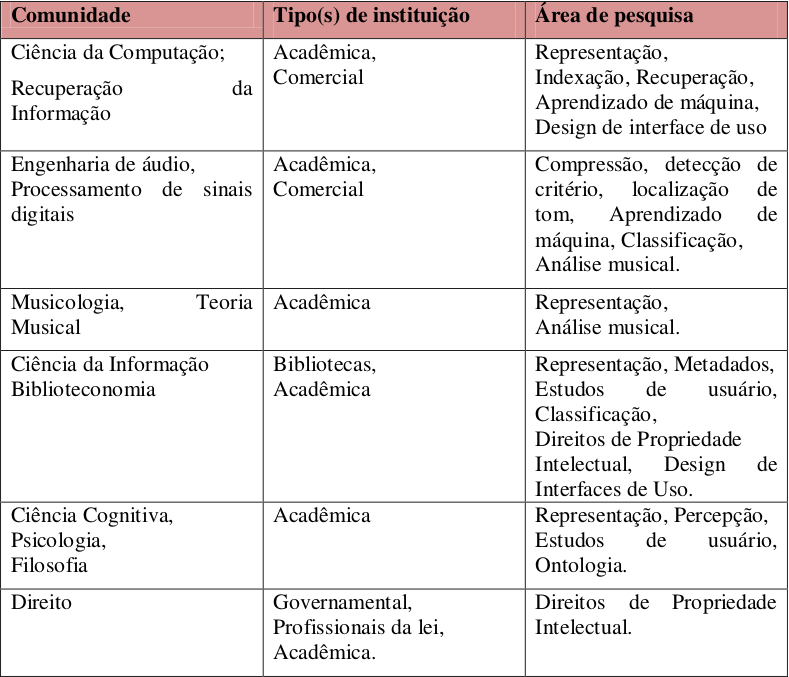
\includegraphics[scale=0.4]{figuras/comunidadeRim.png}
   Fonte: \cite{futrelle&downie2002}.
\end{figure}

A origem de RIM não apresenta uma ação interdisciplinar, o que prejudica todo o seu processo de comunicação científica. Como pontua \citeonline[p.11]{santini&souza2007}:

\begin{citacao}
(...) não há uma sociedade (inter)disciplinar de RIM; um periódico ou livro-texto fundador onde pessoas interessadas podem adquirir as bases teóricas e práticas de RIM. Com exceção de alguns pequenos encontros interdisciplinares, muitos pesquisadores estão apresentando seus resultados para membros das suas próprias disciplinas. A literatura de RIM é difícil de ser localizada, lida e estudada, o que dificulta construir e sustentar uma área de pesquisa respeitável, próspera.
\end{citacao}

A escassa produção científica a respeito do tema e as características impostas pelas músicas acarretam em certas dificuldades para sua representação.

Como elucidado no final do item 2.1 desta seção, o ponto de partida para os estudos sobre a música como fonte de informação e tratamento, representação e recuperação foi dado em 1996 por Alexander McLane. Neste mesmo período já era possível identificar o desenvolvimento de tecnologias de compressão de arquivos digitais de música para transmissão na Internet e a popularização da Internet no mundo \cite{santini&souza2007}.

Em seu estudo McLane direciona sua discussão para os grandes problemas relacionados à representação de documentos de música e à recuperação destes documentos. McLane analisa aspectos significantes da música – sua notação e seu som – e propõe algumas ideias para sistemas de recuperação de música, e formaliza a música como informação segundo três visões: visão subjetiva, visão objetiva e visão interpretativa. Segundo o autor, as necessidades dos vários tipos de análises musicais são tão diversas que é preferível considerar três “visões” sobre a representação da obra musical.

Em resumo adaptado, \citeonline{santini&souza2007} apresenta as principais características das visões estabelecidas por \citeonline{mclane1996}.

\begin{itemize}
    \item A visão \textbf{subjetiva} da informação musical se faz por meio do uso do esquema de notação para representação da informação musical. A subjetividade se dá porque a escolha de elementos de notação geralmente representa uma obra em “contexto-dependente” sendo assim a decisão da notação pode incluir ou excluir aspectos particulares da obra.
    \item A visão \textbf{objetiva} está vinculada a audição e ao momento da execução musical. Um som gravado pode ser identificado como visão objetiva da obra musical. A sonoridade se caracteriza como objetiva por não se configurar como uma representação, mas como a obra em sua essência. O som musical uma vez gravado torna-se fixo e não está mais sujeito a variações editoriais e de performance. Segundo McLane esta visão pode ser considerada a mais completa representação da música, ao passo em que inclui as facetas: tom, tempo, harmonia, editorial e timbre.
    \item A visão \textbf{interpretativa} é realizada através da análise de alguns aspectos da obra, engloba informações que não são diretamente dependentes do documento. Entram nessa categoria classificações e esquemas analíticos que elucidam características como o gênero musical e avaliações críticas.
\end{itemize}

De acordo com \citeonline[p.11]{cruz2014}:

\begin{citacao}
Dentre as visões propostas por McLane (1996), a interpretativa possui uma característica interessante porque permite a independência formal do documento musical em relação ao suporte que o contém, assim como foi possível na informação textual.
\end{citacao}

Segundo \citeonline[p.5]{mclane1996,santini&souza2007}, a representação da informação musical pode abranger as três visões apresentadas dependendo das necessidades de informação da comunidade usuária. De acordo com tradução das autoras, a conclusão de McLane seria a de que:

\begin{citacao}
Ambas as escolhas sobre a visão da representação da música e o grau de complementação da representação de uma obra depende da necessidade de informação do usuário. A recuperação de informação é um processo interativo que depende do conhecimento do usuário e do nível de complexidade da informação desejada. No caso da necessidade da simples identificação de uma obra musical, onde a informação bibliográfica não é unicamente suficiente, pode-se limitar a uma visão subjetiva envolvendo um subconjunto relativamente pequeno de elementos notados de uma obra, frequentemente o tom inicial de uma frase melódica. A representação tonal pode ser de forma tal que provavelmente o usuário espera e está apto para formular a indagação usando a mesma terminologia, ou pelo menos uma que é traduzível na forma de representação.
\end{citacao}

Sendo assim, percebe-se que a recuperação da informação da música depende tanto da complexidade e da forma como a informação é representada como do nível de conhecimento prévio do usuário. Para \citeonline[p.5]{santini&souza2007}: “Quanto menor o conhecimento do usuário, maior a necessidade de diferentes formas de representação. Cada visão da representação da música, demonstrada por McLane, não é suficiente isoladamente para identificar uma obra.”.

Outro autor presente nos estudos relacionados à representação e recuperação de informação musical e um dos representantes da área de RIM é o professor J. Stephen Downie da Universidade de Illinois, nos Estados Unidos. Downie escreveu, em 2003, outro artigo tido como marco no estudo da informação musical, intitulado Music Information Retrieval também em um capítulo do ARIST. No trabalho em questão, \citeonline{downie2003} examina a multidisciplinaridade da área de RIM, identifica e explica alguns problemas relacionados a questão da representação e recuperação da informação musical. Para isso \citeonline{downie2003} resume a questão em quatro grandes desafios a serem enfrentados pelos pesquisadores da área.

De acordo com \citeonline[p.5]{downie2003,santini&souza2007} os quatro desafios seriam:

\begin{citacao}
    \begin{enumerate}
        \item Considerar permanentemente as diferentes formas de representação da música, o que caracteriza o “desafio multirepresentacional”. O copyright faz parte deste desafio.
        \item Cada época histórica e cada formação cultural criam modos próprios e singulares de se expressar através da música. A música transcende as fronteiras culturais e temporais. A ampla variedade de expressões musicais coloca em evidência o “desafio multicultural”.
        \item Compreender e responder às diferentes formas de interação individual com a música e com os siste mas de RIM constitui o “desafio multiexperimental”.
        \item Maximizar os benefícios de ter uma comunidade multidisciplinar de pesquisadores, enquanto minimiza a desvantagem inerente, representa o “desafio multidisciplinar”.
    \end{enumerate}
\end{citacao}

O desafio multirepresentacional é dividido em sete facetas a serem consideradas na descrição da música e que representam a estrutura musical \cite{downie2003}. São elas: tonal, temporal, harmônica, de timbre, editorial, textual e faceta bibliográfica. Sendo as quatro primeiras relativas a aspectos sonoros da música com formas gráficas de representação em figuras rítmicas ou notações musicais, enquanto que as três últimas são representadas na forma gráfica e dizem respeito às informações de produção, intérprete, compositor, copyright, data de produção e outras \cite{barros2012}.

Apesar de completas, a interação dessas facetas resulta em um complexo tratamento da informação musical, visto que cada faceta citada possui por si só uma complexidade inerente e sofre um tipo de representação enquanto produto. As autoras \citeonline[p.8]{santini&souza2007} resumem a problemática multirepresentacional da seguinte forma:

\begin{citacao}
    A complexa interação entre as facetas da música - tempo, harmonia, timbre, freqüência, editoria, texto e bibliografia – evidencia um dos principais problemas de RIM: o desafio multirepresentacional. A escolha da representação da música – se baseada em símbolos, áudio ou ambos – adiciona-se a diversas questões: como, por exemplo, cada escolha determina a tecnologia, a organização, a recuperação e a interface entre requisitos e capacidades dos sistemas.
\end{citacao}

Sendo assim, apesar de possuir as facetas estabelecidas pelo autor, a estrutura da música incorpora elementos extras que nos permitem defini-la como um objeto informacional mais complexo. Além das facetas definidas por  \citeonline[p.283]{downie2003,cruz2014}, a estrutura musical:

\begin{citacao}
    [...] incorpora elementos adicionais que permitem defini-la como um objeto informacional musical mais amplo, dotado de conteúdo – atributos internos e metadados descritivos – e, de contexto – associações com outros objetos musicais e não musicais, e com situações ou eventos em que este objeto musical está inserido.
\end{citacao}

O segundo desafio (multicultural) nasce da condição inerente à música de ser uma objetivação de algo extremamente subjetivo: a expressão humana. Sendo assim, sofre a interferência de uma grande variedade de fatores, da cultura vigente no momento da produção musical e da localização geográfica desta produção.

O desafio multiexperimental diz respeito à percepção da música como experiência individual ou coletiva capaz de causar diferentes reações em diferentes momentos e situações, de cada mente e humor individual. Neste caso ouvir uma música gravada funciona como “ajuda memória” que traz a tona experiências prazerosas ou dolorosas relacionadas a uma música em especial (DOWNIE, 2003 apud SANTINI; SOUZA, 2007, p. 9). As variações de pessoa para pessoa na forma de apropriação, apreciação e nos tipos de experiências emocionais que a música evoca demonstram de maneira pragmática o desafio multiexperimental.

O quarto e último desafio estabelecido por Downie (2003) é o desafio multidisciplinar. Como citado anteriormente, a diversidade intelectual da comunidade de pesquisadores de RIM é, ao mesmo tempo, uma vantagem e uma adversidade. A heterogeneidade das visões de mundo das disciplinas apresenta um problema particular. Cada disciplina traz suas crenças, práticas, questões de pesquisa e paradigmas de avaliação (DOWNIE, 2003). De acordo com Futrelle e Downie (2002), não há uma aceitação comum dos objetivos, técnicas e resultados obtidos nas pesquisas referentes à informação musical.

Percebe-se por tanto, que se por um lado, a ação multidisciplinar dos pesquisadores envolvidos com o tema possibilita o surgimento de diversos avanços tecnológicos e que a cada dia são divulgadas novas soluções para o tratamento de conteúdos musicais, com algoritmos mais sofisticados, novas formas de indexação de músicas, novos tipos de interfaces de áudio e novas formas de representação musical, em contrapartida, é notável a dificuldade de comunicação entre esses resultados. Nota-se ainda a dificuldade de identificação desses conteúdos musicais, porque a música é complexa e possui um leque de propriedades que possibilitam abordagens, às vezes, contraditórias (CRUZ, 2008).

A análise documental da informação musical para sua representação apresenta complexidades, pois exige diferentes técnicas de extração de informações para distintas formas de apresentação.(DOWNIE, 2003).